
% !TeX root=arXiv.tex
% !TEX TS-program = pdfLatex

%%%%%%%%%%%%%%%%%%%%% EXPERIMENTS %%%%%%%%%%%%%%%%%%%%%%%%%%%%%%%%%%%%%
\section{Experiments}\label{sec.4}

To evaluate our proposed method, we quantitatively compare it  with the state-of-the art methods, as well as an informative baseline on all publicly available benchmarks for relative attributes to our knowledge. Furthermore, we perform multiple qualitative experiments to show the %ability
capability and superiority of our method.

\subsection{Datasets}\label{sec.4.1}

To assess the performance of the proposed method, we have evaluate it on all publicly available datasets to our knowledge: \textbf{Zappos50K} \cite{Yu2014} (both coarse and fine-grained versions), \textbf{LFW-10} \cite{Sandeep_2014_CVPR} and for the sake of completeness and comparison with previous works, on \textbf{PubFig} and \textbf{OSR} datasets of \cite{parikh2011}.

\textbf{UT-Zap50K} \cite{Yu2014} dataset is a collection of images with annotations for relative comparison of 4 attributes. This dataset contains two collections: Zappos50K-1, in which relative attributes are annotated for coarse pairs, where the comparisons are relatively easy to interpret, and Zappos50K-2, where relative attributes are annotated for fine-grained pairs, for which making the distinction between them is hard according to human annotators.
Training set for Zappos50K-1 contains approximately 1500 to 1800 annotated pairs of images for each attribute. These are divided into 10 train/test splits which are provided alongside the dataset and used in this work. Meanwhile, Zappos50K-2 only contains a test set of approximately 4300 pairs, which are used for training the set of images in Zappos50K-1.
% This dataset consists of two collections, namely UT-Zap50K-1, in which \textit{coarse} relative attributes are compared for image pairs, and UT-Zap50K-2, in which \textit{fine-grained} relative attributes are compared for image pairs.

We have also conducted experiments on the \textbf{LFW-10} \cite{Sandeep_2014_CVPR} dataset. This dataset has 2000 images of faces of people and annotations for 10 attributes. For each attribute, a random subset of 500 pairs of images have been annotated for each train and test set.
% These two latter datasets have large number of categories, as well as large inter-sample varieties in terms of poses, lighting condition. This makes them quite challenging compared to PubFig and OSR.

\textbf{PubFig} \cite{parikh2011} dataset (a set of public figure faces), consists of 800 facial images of 8 random subjects, with 11 attributes.
\textbf{OSR} \cite{parikh2011} dataset contains 2688 images of outdoor scenes in 8 categories, for which 6 relative attributes are defined.
The ordering of samples in both PubFig and OSR datasets are annotated in a category level, \ie, all images in a specific category may be ranked higher, equal, or lower than all images in another category, with respect to an attribute. This sometimes causes annotation inconsistencies \cite{Sandeep_2014_CVPR}.
In our experiments, we have used the provided train/test split of PubFig and OSR datasets.


\subsection{Experimental setup}
We train our proposed model (described in Section \ref{sec.3}) for each attribute, separately. In our proposed model, it is possible  to train multiple attributes at the same time, however, this is not done due to the structure of datasets, where for each training pair of images only a certain attribute is annotated.

We have used the Lasagne \cite{lasagne} deep learning framework to implement our model.
In all our experiments, for the feature learning and extraction part of the network,
%we use layer fc7 of VGG-16 model of \cite{verydeep} (the last layer before the probability layer).
we use the VGG-16 model of \cite{verydeep} and trim out the probability layer (all layers up to fc7 are used, only the probability layer is not included).
We initialize the weights of the model using a pretrained model on ILSVRC 2014 dataset \cite{ilsvrc2014} for the task of image classification. These weights are fine-tuned as the network learns to predict the relative attributes (see section \ref{sec.qres}). The weights $w$ of the ranking layer are initialized using the Xavier method \cite{glorot}, and the bias is initialized to 0.

For training, we use stochastic gradient descent with RMSProp \cite{Tieleman2012} updates and minibatches of size 32 (16 pair of images).
We set the learning rate for all experiments to $10^{-4}$ (for all weights and biases both the feature learning and extraction layers and the ranking layer), initially, then RMSProp changes the learning rates according to its algorithm. We have also used weight decay ($\ell_2$ norm regularization), with a fixed $0.005$ multiplier. Furthermore, when calculating the binary cross entropy loss, we clip the estimated posterior $p_{ij}$ to be in the range $[10^{-7}, 1 - 10^{-7}]$. This is used to prevent the loss from diverging.

In each epoch, we randomly shuffle the training pairs. The number of epochs of training were chosen to reflect the training size. For Zappos50K and LFW-10 datasets, we train for 5 and 50 epochs, respectively. For PubFig and OSR datasets, we train for 120 epochs due to the small number of training samples. Also, we have added random horizontal flipping of the training images as a way to augment the training set for the PubFig and OSR datasets.

\subsection{Baseline}

As a baseline, we have also included results for the RankSVM method (as in \cite{parikh2011}), when the features given to the method were computed from the output of the VGG-16 pretrained network on ILSVRC 2014. 

Using this baseline we can evaluate the extent of effectiveness of off-the-shelf ConvNet features \cite{offtheshelf}  for the task of ranking. In a sense, comparing this baseline with our proposed method reveals the effect of features fine-tuning, for the task. 

\subsection{Quantitative Results}

 
Following \cite{parikh2011, Yu2014, Sandeep_2014_CVPR}, we report the accuracy in terms of the percentage of correctly ordered pairs. For our proposed method, we report the mean accuracy and standard deviation over 3 separate runs. 
%For a complete report on the results including the standard deviation of the results see supplementary materials.

Table \ref{tab:osr} shows our results on the OSR dataset. Our method outperforms the baseline and the state-of-the-art on this dataset, on all attributes except for `Natural' attribute, where the baseline outperforms our method with a small margin. One possible cause of this could be that the pretrained network of the baseline is still appropriate for this dataset, since the dataset contains natural images. This is a relatively easy dataset, and we would assume that it cannot show the ability of our method to learn better features.

%%%%%%%%%%%%%%%%%%%%%% OSR RESULTS %%%%%%%%%%%%%%%%%%%%%
\begin{table*}[t!]
\caption{Results for the OSR dataset}
\centering
\resizebox{2\columnwidth}{!}{
\begin{tabular}{l| c | c | c | c | c | c | c }
\textbf{Method} & \textbf{Natural} & \textbf{Open} &  \textbf{Perspective} & \textbf{Large Size} & \textbf{Diag} & \textbf{ClsDepth} & \textbf{Mean}\\ \hline
 Relative Attributes~\cite{parikh2011} &  95.03 & 90.77 & 86.73 & 86.23 & 86.50 & 87.53 & 88.80 \\
 Relative Forest~\cite{Li2013} & 95.24 & 92.39 & 87.58 & 88.34 & 89.34 & 89.54 & 90.41 \\
 Fine-grained Comparison~\cite{Yu2014} & 95.70 & 94.10 & 90.43 & 91.10 & 92.43 & 90.47 & 92.37 \\
 VGG16-fc7 (baseline) & 97.98 & 87.82 & 89.01 & 88.25 & 89.91 & 90.70 & 90.61 \\
 %RankNet (ours) & 97.76 ($\pm$ 0.25) & 94.48 ($\pm$ 0.90) & 92.37 ($\pm$ 0.34) & 92.70 ($\pm$ 1.01) & 95.14 ($\pm$ 0.26) & 91.44 ($\pm$ 2.69) & \textbf{93.98} ($\pm$ 0.35) \\
 \hline
 \multirow{2}{*}{RankNet (ours)} & 97.76  & 94.48  & 92.37  & 92.70  & 95.14  & 91.44  & \textbf{93.98}  \\
        & \scriptsize{($\pm$ 0.25)} & \scriptsize{($\pm$ 0.90)} & \scriptsize{($\pm$ 0.34)} & \scriptsize{($\pm$ 1.01)} & \scriptsize{($\pm$ 0.26)} & \scriptsize{($\pm$ 2.69)} & \scriptsize{($\pm$ 0.35)} \\
 \hline
\end{tabular}}
\label{tab:osr}
\end{table*}
%%%%%%%%%%%%%%%%%%%%%%%%%%%%%%%%%%%%%%%%%%%%%%%%%%%%%%%%%

Table \ref{tab:pubfig} shows our results on the PubFig dataset. On this dataset, our results are very competitive with the state-of-the-art. We think this is due to label inconsistency in this dataset, low number of training samples, and the fact that the images in the dataset are very tightly cropped to the face. This makes the decision about the attributes very local, while our method performs the ranking and feature extraction in a global manner.

%%%%%%%%%%%%%%%%%%%%%% PUBFIG RESULTS %%%%%%%%%%%%%%%%%%%
\begin{table*}[t!]
\caption{Results for the PubFig dataset}
\centering
\resizebox{2\columnwidth}{!}{
\begin{tabular}{l|c|c|c|c|c|c|c|c|c|c|c|c}
 \textbf{Method} & \textbf{Male} & \textbf{White} & \textbf{Young} & \textbf{Smiling} & \textbf{Chubby} & \textbf{Forehead} & \textbf{Eyebrow} & \textbf{Eye} & \textbf{Nose} & \textbf{Lip} & \textbf{Face} & \textbf{Mean}  \\ \hline
 Relative Attributes~\cite{parikh2011} & 81.80 & 76.97 & 83.20 & 79.90 & 76.27 & 87.60 & 79.87 & 81.67 & 77.40 & 79.17 & 82.33 & 80.53 \\ 
 Relative Forest~\cite{Li2013} & 85.33 & 82.59 & 84.41 & 83.36 & 78.97 & 88.83 & 81.84 & 83.15 & 80.43 & 81.87 & 86.31 & 83.37 \\
 Fine-grained Comparison~\cite{Yu2014} & 91.77 & 87.43 & 91.87 & 87.00 & 87.37 & 94.00 & 89.83 & 91.40 & 89.07 & 90.43 & 86.70 & \textbf{89.72} \\
 VGG16-fc7 (baseline) & 80.84 & 73.39 & 79.41 & 76.23 & 74.69 & 80.52 & 75.38 & 77.78 & 76.15 & 78.14 & 80.01 & 77.50 \\
 %RankNet (ours) & \pbox{20cm}{\centering 90.10\\($\pm$ 1.05)} & 89.49 ($\pm$ 0.59) & 89.83 ($\pm$ 0.37) & 88.62 ($\pm$ 1.59) & 88.72 ($\pm$ 0.75) & 9.33 ($\pm$ 0.80) & 88.13 ($\pm$ 1.83) & 86.94 ($\pm$ 3.36) & 86.30 ($\pm$ 1.60) & 89.79 ($\pm$ 0.45) & 92.71 ($\pm$ 1.87) & \textbf{89.36 ($\pm$ 0.57)} \\
 \hline
 \multirow{2}{*}{RankNet (ours)} & 90.10 & 89.49 & 89.83 & 88.62 & 88.72 & 92.33 & 88.13 & 86.94 & 86.30 & 89.79 & 92.71 & \textbf{89.36} \\
                                 & \scriptsize{($\pm$ 1.05)} & \scriptsize{($\pm$ 0.59)} & \scriptsize{($\pm$ 0.37)} & \scriptsize{($\pm$ 1.59)} & \scriptsize{($\pm$ 0.75)} & \scriptsize{($\pm$ 0.80)} &  \scriptsize{($\pm$ 1.83)} & \scriptsize{($\pm$ 3.36)} & \scriptsize{($\pm$ 1.60)} & \scriptsize{($\pm$ 0.45)} & \scriptsize{($\pm$ 1.87)} & \scriptsize{($\pm$ 0.57)} \\
 \hline
\end{tabular}}
\label{tab:pubfig}
\end{table*}
%%%%%%%%%%%%%%%%%%%%%%%%%%%%%%%%%%%%%%%%%%%%%%%%%%%%%%%%

Table \ref{tab:lfw} shows our results on the LFW-10 dataset. On this dataset, our method outperforms the state-of-the-art by a large margin. Meanwhile, the baseline cannot achieve a comparative result. This shows that for achieving good results, the feature learning and extraction part have had a large impact.

%%%%%%%%%%%%%%%%%%%%%%% LFW-10 RESULTS %%%%%%%%%%%%%%%%%%
\begin{table*}[t!]
\caption{Results for the LFW-10 dataset}
\centering
\resizebox{2\columnwidth}{!}{
\begin{tabular}{l|c|c|c|c|c|c|c|c|c|c|c}
 \textbf{Method} & \textbf{Bald} & \textbf{DkHair} & \textbf{Eyes} & \textbf{GdLook} & \textbf{Mascu.} & \textbf{Mouth} & \textbf{Smile} & \textbf{Teeth} & \textbf{FrHead} & \textbf{Young} & \textbf{Mean} \\ \hline
 Fine-grained Comparison~\cite{Li2013} & 67.9 & 73.6 & 49.6 & 64.7 & 70.1 & 53.4 & 59.7 & 53.5 & 65.6 & 66.2 & 62.4  \\
 Relative Attributes~\cite{parikh2011} & 70.4 & 75.7 & 52.6 & 68.4 & 71.3 & 55.0 & 54.6 & 56.0 & 64.5 & 65.8 & 63.4 \\
 Relative Parts~\cite{Sandeep_2014_CVPR} & 71.8 & 80.5 & 90.5 & 77.6 & 67.0 & 77.6 & 81.3 & 76.2 & 80.2 & 82.4 & 78.5 \\
 Global + HOG~\cite{vermaexploring} & 78.8 & 72.4 & 70.7 & 67.6 & 84.5 & 67.8 & 67.4 & 71.7 & 79.3 & 68.4 & 72.9 \\
 VGG16-fc7 (baseline) & 70.44 & 69.14 & 59.40 & 59.75 & 84.48 & 56.04 & 57.63 & 57.85 & 59.38 & 70.36 & 64.45 \\
 \hline
 \multirow{2}{*}{RankNet (ours)} & 81.27 & 88.92 & 91.98 & 72.03 & 95.40 & 89.04 & 84.75 & 89.33 & 84.11 & 73.35 & \textbf{85.02} \\ 
                                 & \scriptsize{($\pm$ 1.47)} & \scriptsize{($\pm$ 1.63)} & \scriptsize{($\pm$ 2.42)} & \scriptsize{($\pm$ 1.25)} & \scriptsize{($\pm$ 1.52)} & \scriptsize{($\pm$ 2.18)} & \scriptsize{($\pm$ 0.28)} & \scriptsize{($\pm$ 0.47)} & \scriptsize{($\pm$ 2.77)} & \scriptsize{($\pm$ 1.13)} & \scriptsize{($\pm$ 0.59)} \\
 \hline
\end{tabular}}
\label{tab:lfw}
\end{table*}
%%%%%%%%%%%%%%%%%%%%%%%%%%%%%%%%%%%%%%%%%%%%%%%%%%%%%%%%

Tables \ref{tab:zap1} and \ref{tab:zap2} show the results on Zappos50K-1 and Zappos50K-2 datasets, respectively. Our method, again, achieves the state-of-the-art accuracy on both fine-grained and coarse-grained datasets. However, our baseline method does not achieve a good result on this dataset. We would assume this is due to the fact that the images in the Zappos50K dataset are not natural images. So the extracted features in the baseline method are not appropriate for ranking. But our proposed method learns appropriate features for the task, given the large amount of training data available in this dataset.

%%%%%%%%%%%%%%%%%%%%%% Zap50K-1 RESULTS %%%%%%%%%%%%%%%%
\begin{table}[h]
\caption{Results for the UT-Zap50K-1 (coarse) dataset}
%\centering
\resizebox{1\columnwidth}{!}{
\begin{tabular}{l|c|c|c|c|c}
 \textbf{Method} & \textbf{Open} & \textbf{Pointy} & \textbf{Sporty} & \textbf{Comfort} & \textbf{Mean} \\ \hline
 Relative Attributes~\cite{parikh2011} & 87.77 & 89.37 & 91.20 & 89.93 & 89.57 \\
 Fine-grained Comparison~\cite{Yu2014} & 90.67 & 90.83 & 92.67 & 92.37 & 91.64 \\
 VGG16-fc7 (baseline) & 62.33 & 59.57 & 61.33 & 61.00 & 61.08 \\
 \hline
 \multirow{2}{*}{RankNet (ours)} & 93.00 & 92.11 & 95.56 & 93.22 & \textbf{93.47}\\
                                 & \scriptsize{($\pm$ 1.15)} & \scriptsize{($\pm$ 1.58)} & \scriptsize{($\pm$ 1.26)} & \scriptsize{($\pm$ 2.41)} & \scriptsize{($\pm$ 0.59)}\\
 \hline
\end{tabular}}
\label{tab:zap1}
\end{table}
%%%%%%%%%%%%%%%%%%%%%%%%%%%%%%%%%%%%%%%%%%%%%%%%%%%%%%%%


%%%%%%%%%%%%%%%%%%%%%% Zap50K-2 RESULTS %%%%%%%%%%%%%%%%
\begin{table}[h]
\caption{Results for the UT-Zap50K-2 (fine-grained) dataset}
%\centering
\resizebox{\columnwidth}{!}{
\begin{tabular}{l|c|c|c|c|c}
 \textbf{Method} & \textbf{Open} & \textbf{Pointy} & \textbf{Sporty} & \textbf{Comfort} & \textbf{Mean} \\ \hline
 Relative Attributes~\cite{parikh2011} & 60.18 & 59.56 & 62.70 & 64.04 & 61.62  \\
 Fine-grained Comparison~\cite{Yu2014} & 74.91 & 63.74 & 64.54 & 62.51 & 66.43  \\
 LocalPair + ML + HOG~\cite{vermaexploring} & 76.2 & 65.3 & 64.8 & 63.6 & 67.5 \\
 VGG16-fc7 (baseline) & 52.55 & 52.65 & 51.52 & 53.01 & 52.43 \\
 \hline
 \multirow{2}{*}{RankNet (ours)} & 71.21 & 66.64 & 67.81 & 65.88 & \textbf{67.88} \\
                                 & \scriptsize{($\pm$ 1.50)} & \scriptsize{($\pm$ 1.81)} & \scriptsize{($\pm$ 0.84)} & \scriptsize{($\pm$ 1.92)} & \scriptsize{($\pm$ 0.83)}\\
 \hline
\end{tabular}}
\label{tab:zap2}
\end{table}
%%%%%%%%%%%%%%%%%%%%%%%%%%%%%%%%%%%%%%%%%%%%%%%%%%%%%%%%

\subsection{Qualitative Results} \label{sec.qres}


%%%%%%%%%%%%%%%%%%%%% Figure featspace %%%%%%%%%%%%%%%%%%%%%%%%%%%%%%%%
\begin{figure*}
\resizebox{2\columnwidth}{!}{
\centering
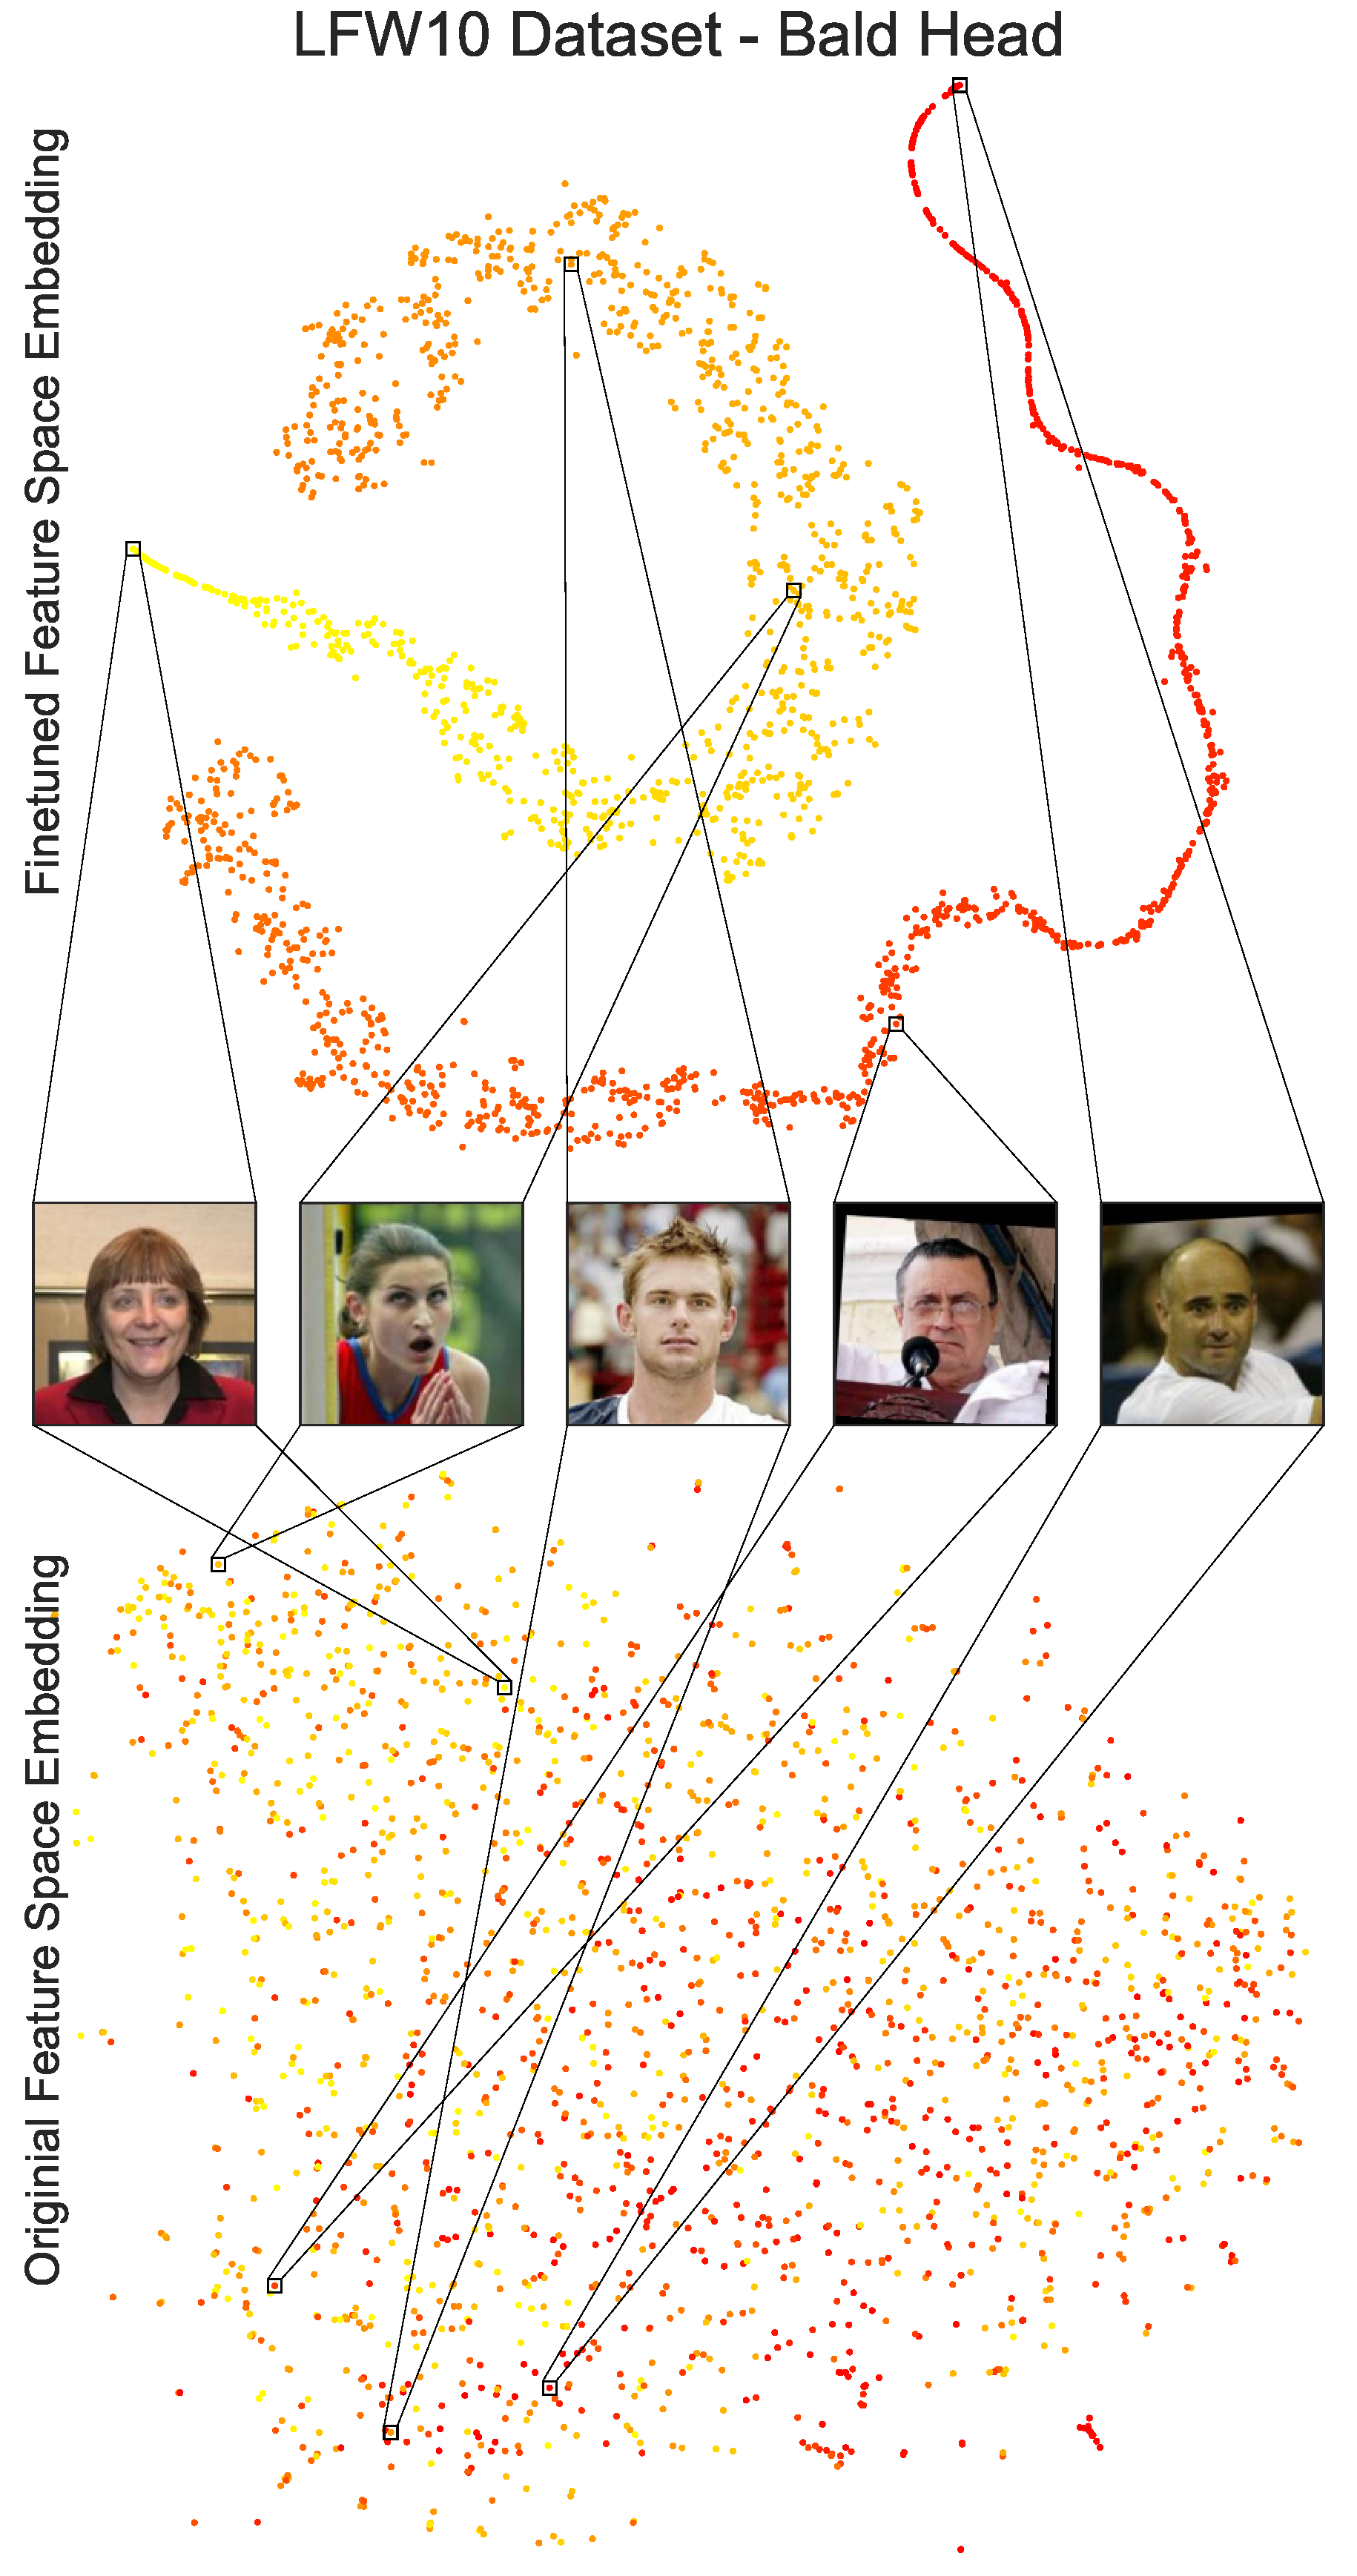
\includegraphics{lfw10-baldhead-featspace.pdf}
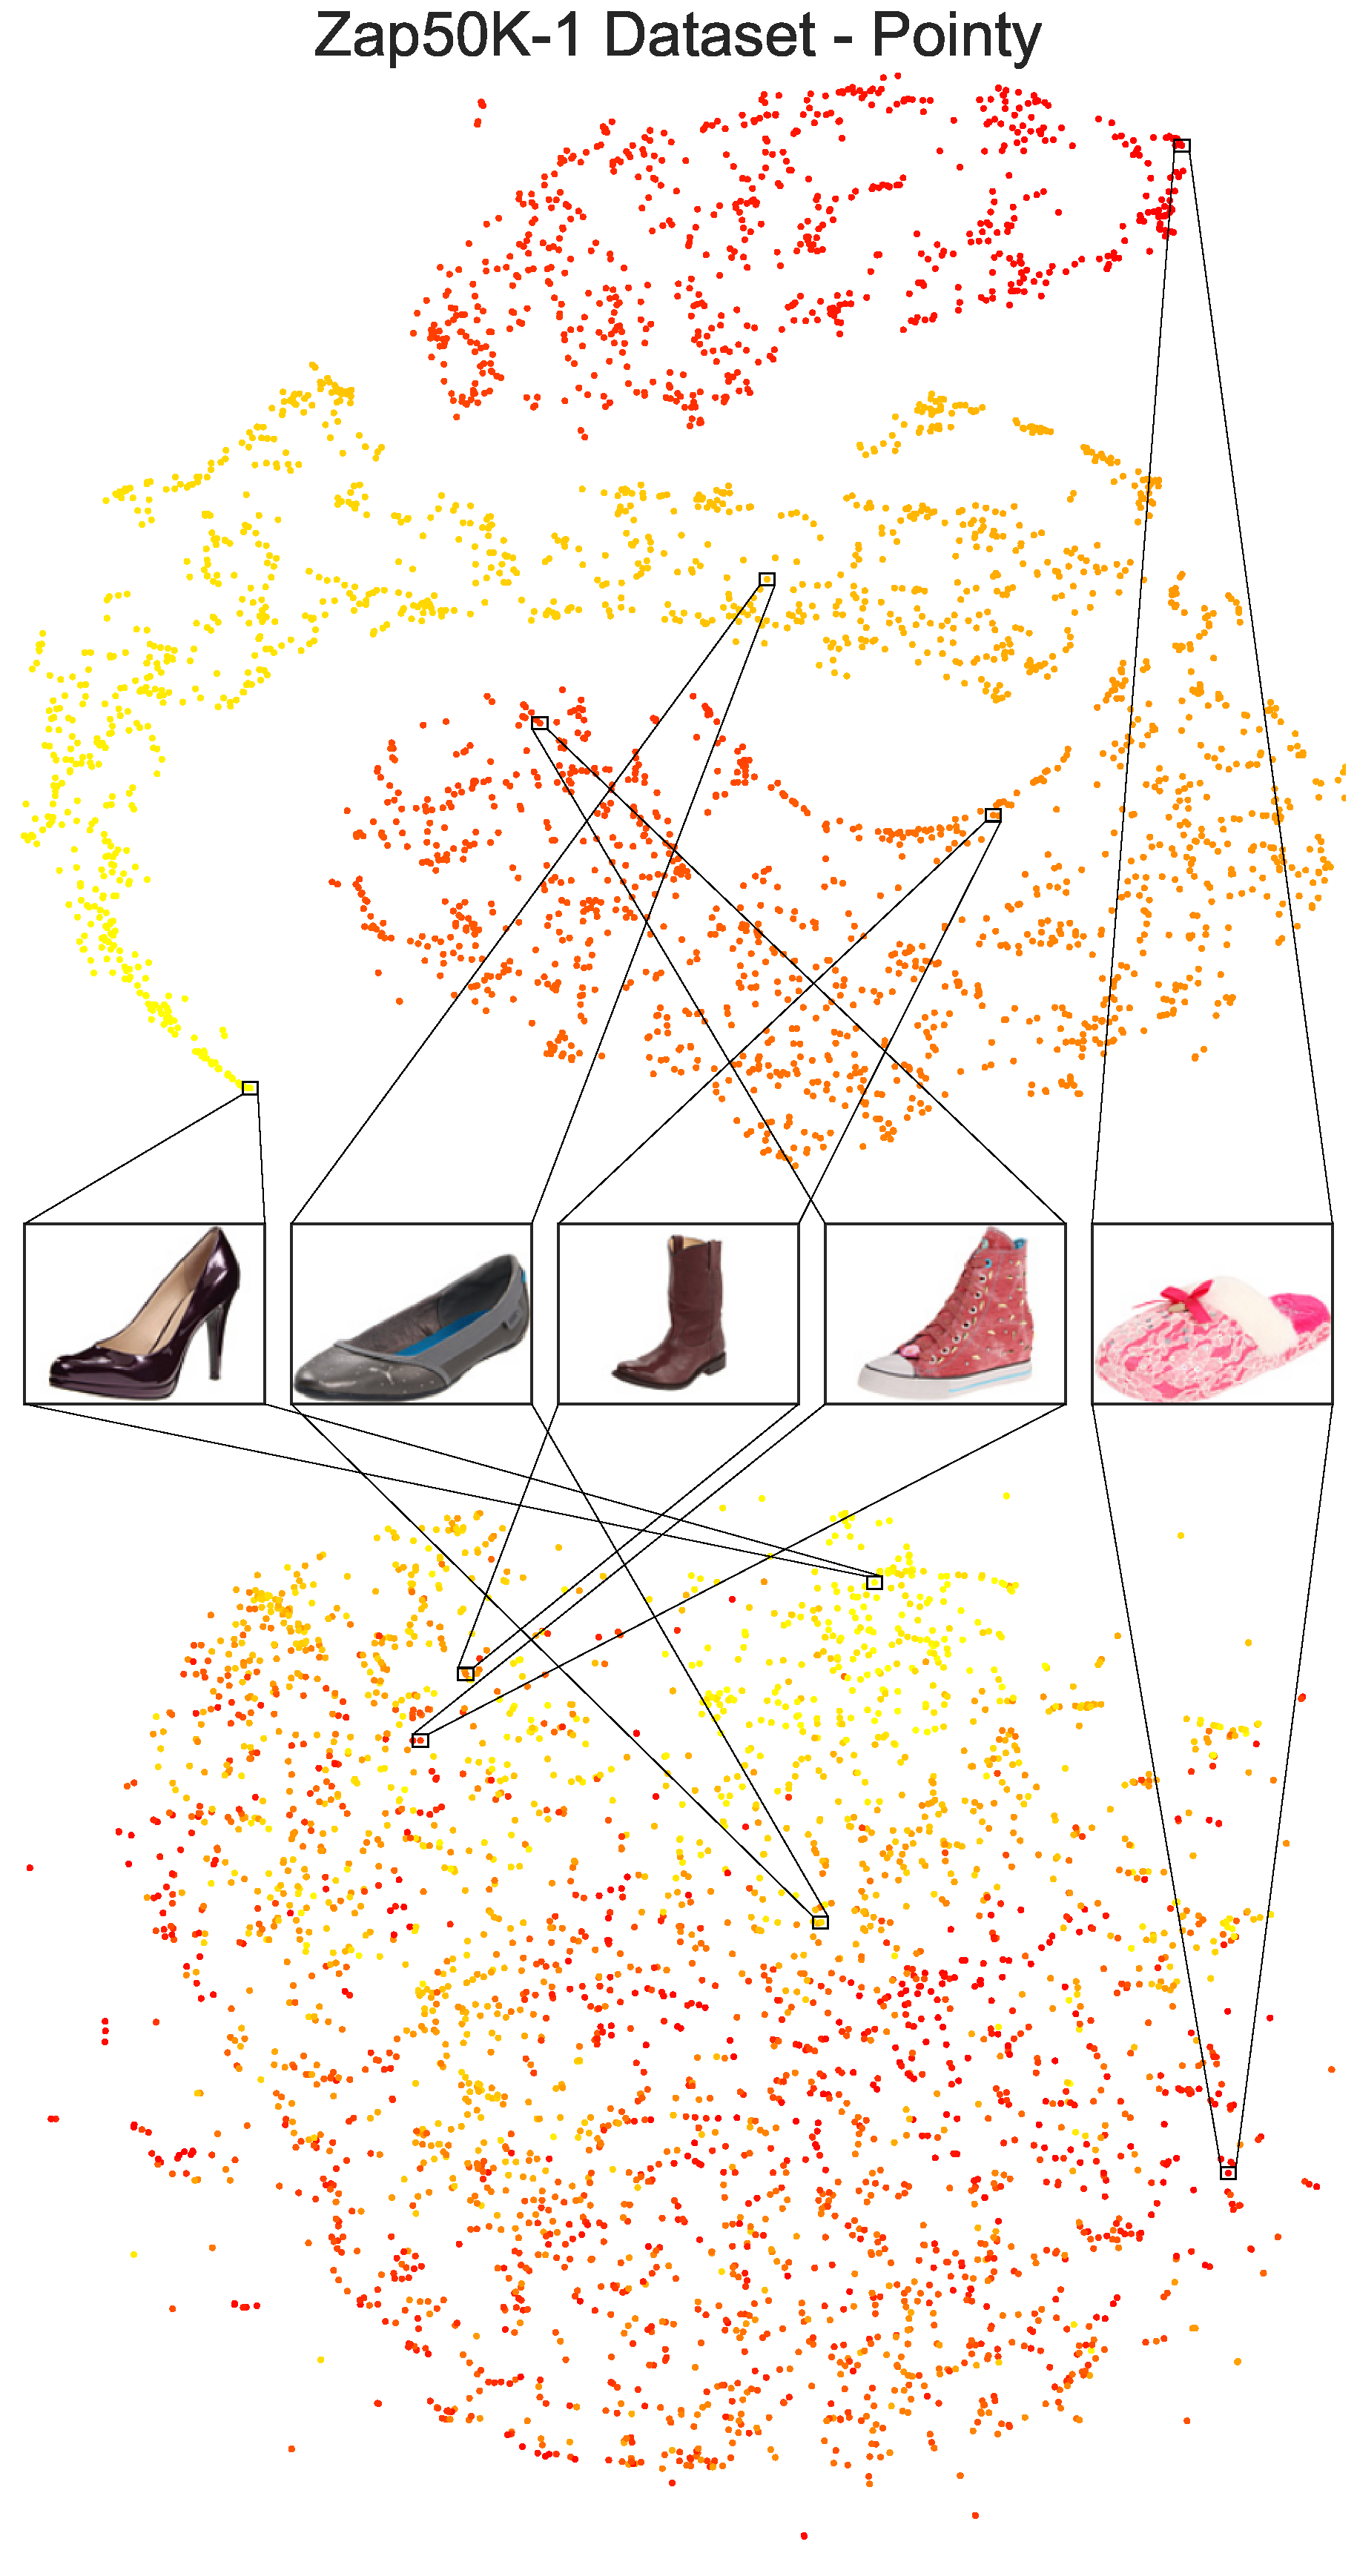
\includegraphics{zappos-pointy-featspace.pdf}
}
\caption{t-SNE embedding of images in fine-tuned feature space (top) and original feature space (bottom). The set of visualizations on the left are for the \textit{Bald Head} attribute of the LFW-10 dataset. The set of visualizations on the right are for the \textit{Pointy} attribute of the Zappos50K-1 dataset. Images in the middle row show a number of samples from the feature space. It is clear that images are ordered according to their value of the attribute. Each point is colored according to its value of the respective attribute, to discriminate images according to their value of the attribute.}
\label{featspace}
\end{figure*}
%%%%%%%%%%%%%%%%%%%%% Figure featspace %%%%%%%%%%%%%%%%%%%%%%%%%%%%%%%%


%%%%%%%%%%%%%%%%%%%%% Figure 5 %%%%%%%%%%%%%%%%%%%%%%%%%%%%%%%%%%%%%%%%
\begin{figure*}
\scalebox{.38}
{
\begin{tikzpicture}

		\node [scale=2] (strong) {\textit{strong}}; 
	\node [scale=2, right=31cm of strong] (weak) {\textit{weak}};
	\path [draw, line width=3, <->, blue] (strong.south west) -- (weak.south east);

	% attr1
	\node [below=0.5cm of strong] (attr1im1) {
\includegraphics[width=4cm, height=4cm]{spectrum/attr1/im1.jpg}};
	\node (attr1name) [scale=2, left=0.5cm of attr1im1] {Smile (LFW-10)};
	\node [right=0.5cm of attr1im1] (attr1im2) {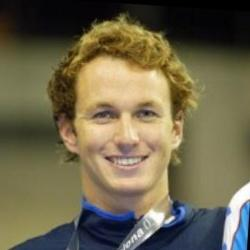
\includegraphics[width=4cm, height=4cm]{spectrum/attr1/im2.jpg}};
	\node [right=0.5cm of attr1im2] (attr1im3) {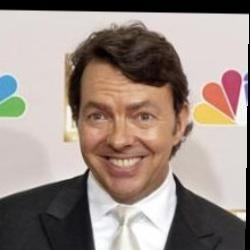
\includegraphics[width=4cm, height=4cm]{spectrum/attr1/im3.jpg}};
	\node [right=0.5cm of attr1im3] (attr1im4) {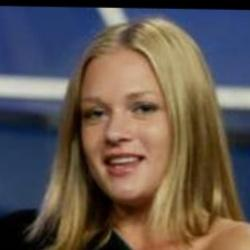
\includegraphics[width=4cm, height=4cm]{spectrum/attr1/im4.jpg}};
	\node [right=0.5cm of attr1im4] (attr1im5) {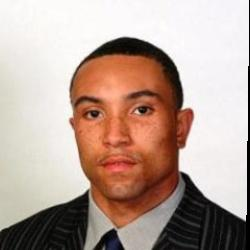
\includegraphics[width=4cm, height=4cm]{spectrum/attr1/im5.jpg}};
	\node [right=0.5cm of attr1im5] (attr1im6) {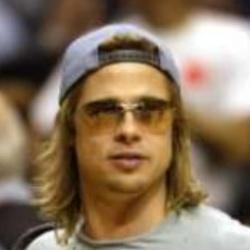
\includegraphics[width=4cm, height=4cm]{spectrum/attr1/im6.jpg}};
	\node [right=0.5cm of attr1im6] (attr1im7) {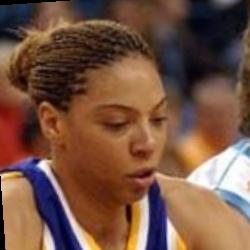
\includegraphics[width=4cm, height=4cm]{spectrum/attr1/im7.jpg}};
	\node [right=0.5cm of attr1im7] (attr1im8) {
\includegraphics[width=4cm, height=4cm]{spectrum/attr1/im8.jpg}};

% 	% attr2
% 	\node [below=0.5cm of attr1im1] (attr2im1) {
\includegraphics[width=4cm, height=4cm]{spectrum/attr2/im1.jpg}};
% 	\node (attr2name) [scale=2, left=0.5cm of attr2im1] {Young};
% 	\node [right=0.5cm of attr2im1] (attr2im2) {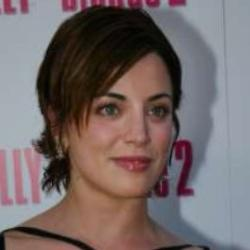
\includegraphics[width=4cm, height=4cm]{spectrum/attr2/im2.jpg}};
% 	\node [right=0.5cm of attr2im2] (attr2im3) {
\includegraphics[width=4cm, height=4cm]{spectrum/attr2/im3.jpg}};
% 	\node [right=0.5cm of attr2im3] (attr2im4) {
\includegraphics[width=4cm, height=4cm]{spectrum/attr2/im4.jpg}};
% 	\node [right=0.5cm of attr2im4] (attr2im5) {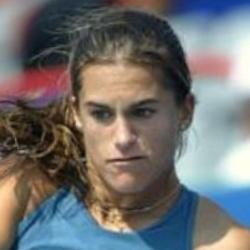
\includegraphics[width=4cm, height=4cm]{spectrum/attr2/im5.jpg}};
% 	\node [right=0.5cm of attr2im5] (attr2im6) {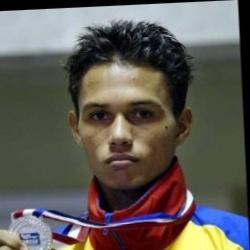
\includegraphics[width=4cm, height=4cm]{spectrum/attr2/im6.jpg}};
% 	\node [right=0.5cm of attr2im6] (attr2im7) {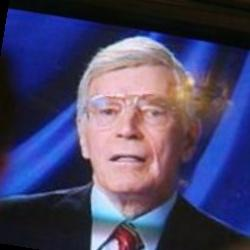
\includegraphics[width=4cm, height=4cm]{spectrum/attr2/im7.jpg}};
% 	\node [right=0.5cm of attr2im7] (attr2im8) {
\includegraphics[width=4cm, height=4cm]{spectrum/attr2/im8.jpg}};

% 	% attr3
% 	\node [below=0.5cm of attr2im1] (attr3im1) {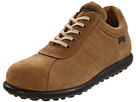
\includegraphics[width=4cm, height=3cm]{spectrum/attr3/im1.jpg}};
% 	\node (attr3name) [scale=2, left=0.5cm of attr3im1] {Comfort};
% 	\node [right=0.5cm of attr3im1] (attr3im2) {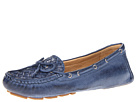
\includegraphics[width=4cm, height=3cm]{spectrum/attr3/im2.jpg}};
% 	\node [right=0.5cm of attr3im2] (attr3im3) {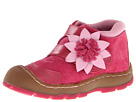
\includegraphics[width=4cm, height=3cm]{spectrum/attr3/im3.jpg}};
% 	\node [right=0.5cm of attr3im3] (attr3im4) {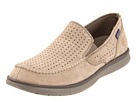
\includegraphics[width=4cm, height=3cm]{spectrum/attr3/im4.jpg}};
% 	\node [right=0.5cm of attr3im4] (attr3im5) {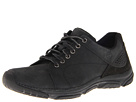
\includegraphics[width=4cm, height=3cm]{spectrum/attr3/im5.jpg}};
% 	\node [right=0.5cm of attr3im5] (attr3im6) {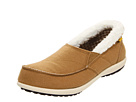
\includegraphics[width=4cm, height=3cm]{spectrum/attr3/im6.jpg}};
% 	\node [right=0.5cm of attr3im6] (attr3im7) {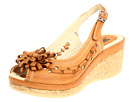
\includegraphics[width=4cm, height=3cm]{spectrum/attr3/im7.jpg}};
% 	\node [right=0.5cm of attr3im7] (attr3im8) {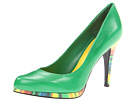
\includegraphics[width=4cm, height=3cm]{spectrum/attr3/im8.jpg}};

	% attr4
	\node [below=0.5cm of attr1im1] (attr4im1) {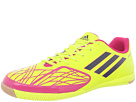
\includegraphics[width=4cm, height=3cm]{spectrum/attr4/im1.jpg}};
	\node (attr4name) [scale=2, left=0.5cm of attr4im1] {Sporty (Zappos50K-1)};
	\node [right=0.5cm of attr4im1] (attr4im2) {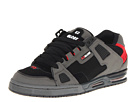
\includegraphics[width=4cm, height=3cm]{spectrum/attr4/im2.jpg}};
	\node [right=0.5cm of attr4im2] (attr4im3) {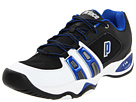
\includegraphics[width=4cm, height=3cm]{spectrum/attr4/im3.jpg}};
	\node [right=0.5cm of attr4im3] (attr4im4) {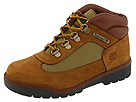
\includegraphics[width=4cm, height=3cm]{spectrum/attr4/im4.jpg}};
	\node [right=0.5cm of attr4im4] (attr4im5) {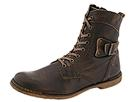
\includegraphics[width=4cm, height=3cm]{spectrum/attr4/im5.jpg}};
	\node [right=0.5cm of attr4im5] (attr4im6) {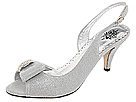
\includegraphics[width=4cm, height=3cm]{spectrum/attr4/im6.jpg}};
	\node [right=0.5cm of attr4im6] (attr4im7) {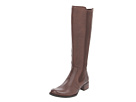
\includegraphics[width=4cm, height=3cm]{spectrum/attr4/im7.jpg}};
	\node [right=0.5cm of attr4im7] (attr4im8) {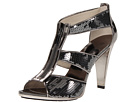
\includegraphics[width=4cm, height=3cm]{spectrum/attr4/im8.jpg}};

	% attr5
	\node [below=0.5cm of attr4im1] (attr5im1) {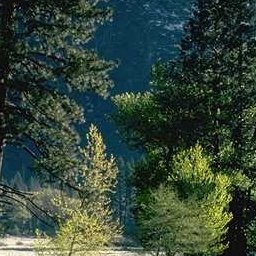
\includegraphics[width=4cm, height=4cm]{spectrum/attr5/im1.jpg}};
	\node (attr5name) [scale=2, left=0.5cm of attr5im1] {Natural (OSR)};
	\node [right=0.5cm of attr5im1] (attr5im2) {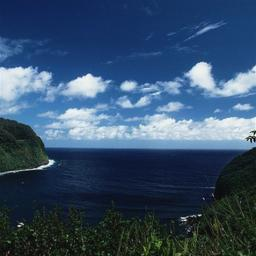
\includegraphics[width=4cm, height=4cm]{spectrum/attr5/im2.jpg}};
	\node [right=0.5cm of attr5im2] (attr5im3) {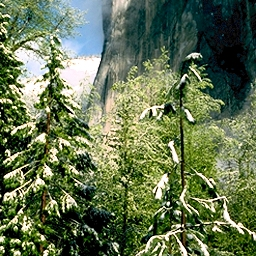
\includegraphics[width=4cm, height=4cm]{spectrum/attr5/im3.jpg}};
	\node [right=0.5cm of attr5im3] (attr5im4) {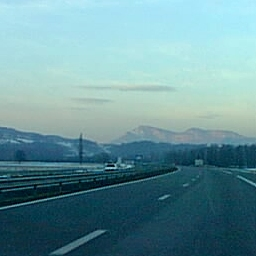
\includegraphics[width=4cm, height=4cm]{spectrum/attr5/im4.jpg}};
	\node [right=0.5cm of attr5im4] (attr5im5) {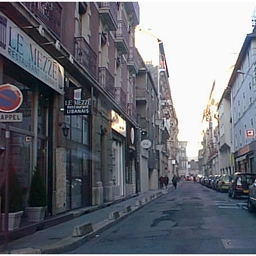
\includegraphics[width=4cm, height=4cm]{spectrum/attr5/im5.jpg}};
	\node [right=0.5cm of attr5im5] (attr5im6) {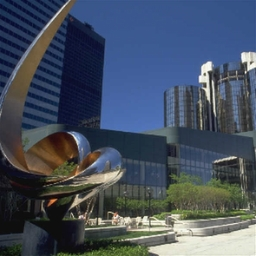
\includegraphics[width=4cm, height=4cm]{spectrum/attr5/im6.jpg}};
	\node [right=0.5cm of attr5im6] (attr5im7) {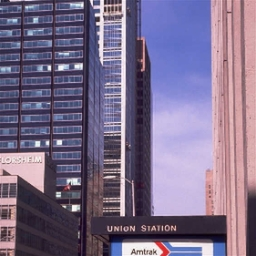
\includegraphics[width=4cm, height=4cm]{spectrum/attr5/im7.jpg}};
	\node [right=0.5cm of attr5im7] (attr5im8) {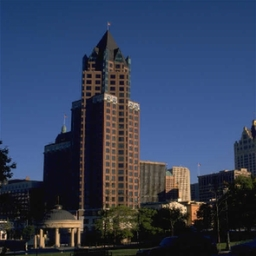
\includegraphics[width=4cm, height=4cm]{spectrum/attr5/im8.jpg}};

% 	% attr6
% 	\node [below=0.5cm of attr5im1] (attr6im1) {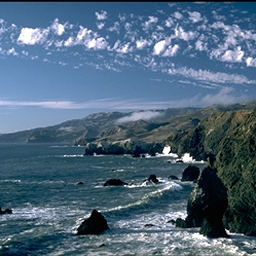
\includegraphics[width=4cm, height=4cm]{spectrum/attr6/im1.jpg}};
% 	\node (attr6name) [scale=2, left=0.5cm of attr6im1] {Open};
% 	\node [right=0.5cm of attr6im1] (attr6im2) {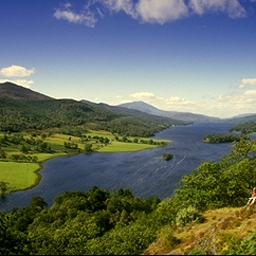
\includegraphics[width=4cm, height=4cm]{spectrum/attr6/im2.jpg}};
% 	\node [right=0.5cm of attr6im2] (attr6im3) {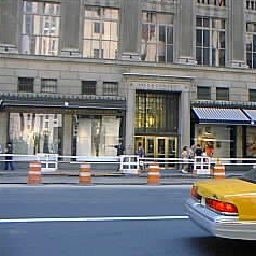
\includegraphics[width=4cm, height=4cm]{spectrum/attr6/im3.jpg}};
% 	\node [right=0.5cm of attr6im3] (attr6im4) {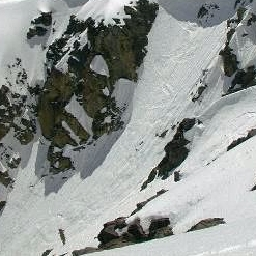
\includegraphics[width=4cm, height=4cm]{spectrum/attr6/im4.jpg}};
% 	\node [right=0.5cm of attr6im4] (attr6im5) {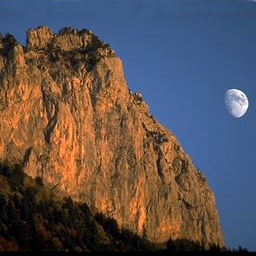
\includegraphics[width=4cm, height=4cm]{spectrum/attr6/im5.jpg}};
% 	\node [right=0.5cm of attr6im5] (attr6im6) {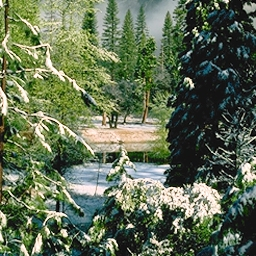
\includegraphics[width=4cm, height=4cm]{spectrum/attr6/im6.jpg}};
% 	\node [right=0.5cm of attr6im6] (attr6im7) {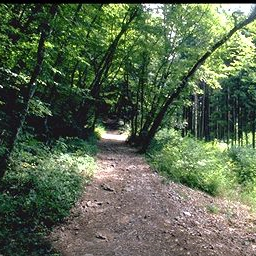
\includegraphics[width=4cm, height=4cm]{spectrum/attr6/im7.jpg}};
% 	\node [right=0.5cm of attr6im7] (attr6im8) {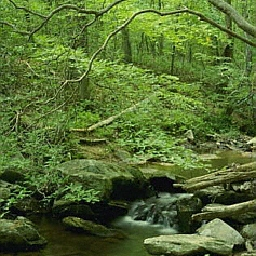
\includegraphics[width=4cm, height=4cm]{spectrum/attr6/im8.jpg}};

	% attr7
	\node [below=0.5cm of attr5im1] (attr7im1) {\includegraphics[width=4cm, height=4cm]{spectrum/attr7/im1.jpg}};
	\node (attr7name) [scale=2, left=0.5cm of attr7im1] {Forehead (PubFig)};
	\node [right=0.5cm of attr7im1] (attr7im2) {\includegraphics[width=4cm, height=4cm]{spectrum/attr7/im2.jpg}};
	\node [right=0.5cm of attr7im2] (attr7im3) {\includegraphics[width=4cm, height=4cm]{spectrum/attr7/im3.jpg}};
	\node [right=0.5cm of attr7im3] (attr7im4) {\includegraphics[width=4cm, height=4cm]{spectrum/attr7/im4.jpg}};
	\node [right=0.5cm of attr7im4] (attr7im5) {\includegraphics[width=4cm, height=4cm]{spectrum/attr7/im5.jpg}};
	\node [right=0.5cm of attr7im5] (attr7im6) {\includegraphics[width=4cm, height=4cm]{spectrum/attr8/im2.jpg}};
	\node [right=0.5cm of attr7im6] (attr7im7) {\includegraphics[width=4cm, height=4cm]{spectrum/attr7/im7.jpg}};
	\node [right=0.5cm of attr7im7] (attr7im8) {\includegraphics[width=4cm, height=4cm]{spectrum/attr7/im8.jpg}};

% 	% attr8
% 	\node [below=0.5cm of attr7im1] (attr8im1) {\includegraphics[width=4cm, height=4cm]{spectrum/attr8/im1.jpg}};
% 	\node (attr8name) [scale=2, left=0.5cm of attr8im1] {Open Eyes};
% 	\node [right=0.5cm of attr8im1] (attr8im2) {\includegraphics[width=4cm, height=4cm]{spectrum/attr8/im2.jpg}};
% 	\node [right=0.5cm of attr8im2] (attr8im3) {\includegraphics[width=4cm, height=4cm]{spectrum/attr8/im3.jpg}};
% 	\node [right=0.5cm of attr8im3] (attr8im4) {\includegraphics[width=4cm, height=4cm]{spectrum/attr8/im4.jpg}};
% 	\node [right=0.5cm of attr8im4] (attr8im5) {\includegraphics[width=4cm, height=4cm]{spectrum/attr8/im5.jpg}};
% 	\node [right=0.5cm of attr8im5] (attr8im6) {\includegraphics[width=4cm, height=4cm]{spectrum/attr8/im6.jpg}};
% 	\node [right=0.5cm of attr8im6] (attr8im7) {\includegraphics[width=4cm, height=4cm]{spectrum/attr8/im7.jpg}};
% 	\node [right=0.5cm of attr8im7] (attr8im8) {\includegraphics[width=4cm, height=4cm]{spectrum/attr8/im8.jpg}};
\end{tikzpicture}}
\caption{Sample images from different datasets, ordered according to the predicted value of their respective attribute.}
\label{figspectrum}
\end{figure*}
%%%%%%%%%%%%%%%%%%%%% Figure 5 %%%%%%%%%%%%%%%%%%%%%%%%%%%%%%%%%%%%%%%%

Our proposed method uses a deep network with two parts, the feature learning and extraction part and the ranking part. During training, not only the weights for the ranking part are learned, but also the weights for the feature learning and extraction part of the network, which were initialized using a pretrained network, are fine-tuned. By fine-tuning the features, our network learns a set of features that are more appropriate for the images of that particular dataset, along with the attribute of interest. To show the effectiveness of fine-tuning the features of the feature learning and extraction part of the network, we have projected them into 2-D space using the t-SNE \cite{van2008visualizing} method, as can be seen in Figure \ref{featspace}. The visualizations on the top of each figure show the images projected into 2-D space from the fine-tuned feature space. Each image is displayed as a point. It is clear from these visualizations that fine-tuned feature space is better in capturing the ordering of images with respect to the respective attribute. Since t-SNE embedding is a non-linear embedding, relative distances between points in the high-dimensional space and the low-dimensional embedding space are preserved, thus close points in the low-dimensional embedding space are also close to each other in the high-dimensional space. It can, therefore, be seen that fine-tuning indeed changes the feature space such that images with similar values of the respective attribute get projected into a close vicinity of the feature space. However, in the original feature space, images are projected according to their visual content, regardless of their value of the attribute.

Another property of our network is that it can achieve a total ordering of images, given a set of pairwise orderings. In spite of the fact that training samples are pairs of images annotated according to their relative value of the attribute, the network can generalize the relativity of attribute values to other pairs of images. Figure \ref{figspectrum} shows that images can be ordered according to their value of the respective attribute. 

\subsection{Saliency Maps and Localizing the Attributes} \label{sec.4.5}

We have also used the method of \cite{saliency} to visualize the saliency of each attribute. Giving two image as inputs to the network, we take the derivative of the estimated posterior with respect to the input images and visualize them. Figure \ref{fig.5} shows some sample visualization for the LFW-10 dataset's test pairs. To generate this figure we have applied Gaussian smoothing to the saliency map.
Using this visualization, we can localize the attribute using the same network that was trained to rank the attributes in an unsupervised manner, \ie, although we haven't explicitly trained our network to localize the salient and informative regions of the image, %however,
it has implicitly learned to find these regions. We see that this technique is able to localize both easy attributes such as "Open Eyes" and abstract attributes such as "Good Looking". Our approach reveals some interesting properties about salient pixels for each attribute. For example, for the attribute "Open Eyes", not only pixels belonging to the eye are salient, but the pixels which belong to the mouth are also salient. This is because the person with open mouth usually has open eyes.

\begin{figure}[th!]
\captionsetup[subfigure]{labelformat=empty}
    \centering
    \begin{subfigure}
        \centering
        \includegraphics[width=8cm, trim={0 1cm 0 0},clip]{saliency-new/saliency-smooth/bald-1.jpeg}
        \footnotesize
        \stackunder[3pt]{
            \includegraphics[width=8cm, trim={0 0 0 1cm},clip]{saliency-new/saliency-smooth/bald-6.jpeg}
        }{Bald Head}
        \vspace{0.4cm}
    \end{subfigure}
    
    \begin{subfigure}
        \centering
        \includegraphics[width=8cm, trim={0 1cm 0 0},clip]{saliency-new/saliency-smooth/smile-1.jpeg}
        \footnotesize
        \stackunder[3pt]{
            \includegraphics[width=8cm, trim={0 0 0 1cm},clip]{saliency-new/saliency-smooth/smile-4.jpeg}
        }{Smile}
        \vspace{0.4cm}
    \end{subfigure}
    
    \begin{subfigure}
        \centering
        \includegraphics[width=8cm, trim={0 1cm 0 0},clip]{saliency-new/saliency-smooth/eyesopen-1.jpeg}
        \footnotesize
        \stackunder[3pt]{
            \includegraphics[width=8cm, trim={0 0 0 1cm},clip]{saliency-new/saliency-smooth/eyesopen-5.jpeg}
        }{Open Eyes}
        \vspace{0.4cm}
    \end{subfigure}
    
    \begin{subfigure}
        \centering
        \includegraphics[width=8cm, trim={0 1cm 0 0},clip]{saliency-new/saliency-smooth/goodlooking-1.jpeg}
        \footnotesize
        \stackunder[3pt]{
            \includegraphics[width=8cm, trim={0 0 0 1cm} ,clip]{saliency-new/saliency-smooth/goodlooking-4.jpeg}
        }{Good Looking}
    \end{subfigure}
    
    \caption{Saliency maps obtained from the network. First we feed two test images into the network and compute the derivative of the estimated posterior with respect to the pair of input images and use the method of \cite{saliency} to visualize salient pixels with  Gaussian smoothing. In each row, the two input images from the LFW-10 test set with their corresponding overlaid saliency maps are shown (the warmer the color of the overlay image, the more salient that pixel is).}
    \label{fig.5}
\end{figure}
